%%%%%%%%%%%%%%%%%%%%%%%%%%%%%%%%%%%%%%%%%%%%%%%%%%%%%%%%%%%%%%%%%%%%%%%%
%     LaTeX source code to approximate a NIST Technical report
%	  Instructions for authors: tinyurl.com/techpubsnist
%	DOI watermark will be added on final PDF
% 	Developed by K. Miller, kmm5@nist.gov
%	Last updated: 10-Oct-2017
%%%%%%%%%%%%%%%%%%%%%%%%%%%%%%%%%%%%%%%%%%%%%%%%%%%%%%%%%%%%%%%%%%%
\documentclass[12pt]{article}
\usepackage{adjustbox}
\usepackage{amsmath}
\usepackage{amsfonts}   % if you want the fonts
\usepackage{amssymb}    % if you want extra symbols
\usepackage{bm}
\usepackage{float}
\usepackage[hang,flushmargin,bottom]{footmisc} % footnote format
\usepackage{graphicx}   % need for figures		
\usepackage{mathptmx}
\usepackage{multicol}
\usepackage{physics}
\usepackage{rotating}
\usepackage{secdot}
\usepackage{siunitx} % Formats the units and values
\usepackage{tabulary}
\usepackage{textgreek}
\usepackage{textcomp}
\usepackage{tikz}
\usepackage{titlesec}
\usepackage[utf8]{inputenc}
\usepackage{xcolor}
\titleformat{\section}{\normalsize\bfseries}{\thesection.}{1em}{}	% required for heading numbering style
\titleformat*{\subsection}{\normalsize\bfseries}

\usepackage{tocloft}	% change typeset, titles, and format list of appendices/figures/tables
\renewcommand{\cftdot}{}	
\renewcommand{\contentsname}{Table of Contents}
\renewcommand{\cftpartleader}{\cftdotfill{\cftdotsep}} % for parts
\renewcommand{\cftsecleader}{\cftdotfill{\cftdotsep}}
\renewcommand\cftbeforesecskip{\setlength{4pt}{}}
\addtolength{\cftfignumwidth}{1em}
\renewcommand{\cftfigpresnum}{\figurename\ }
\addtolength{\cfttabnumwidth}{1em}
\renewcommand{\cfttabpresnum}{\tablename\ }
\setlength{\cfttabindent}{0in}    %% adjust as you like
\setlength{\cftfigindent}{0in}

\usepackage{enumitem}         % to control spacing between bullets/numbered lists

\usepackage[numbers,sort&compress]{natbib} % format bibliography
\renewcommand{\bibsection}{}
\setlength{\bibsep}{0.0pt}

\usepackage[hidelinks]{hyperref} % hyperref package & removing outline from links

\usepackage{epstopdf} % converting EPS figure files to PDF

\usepackage{fancyhdr, lastpage}	% formatting document, calculating number of pages, formatting headers
\setlength{\topmargin}{-0.5in}
\setlength{\headheight}{39pt}
\setlength{\oddsidemargin}{0.25in}
\setlength{\evensidemargin}{0.25in}
\setlength{\textwidth}{6.0in}
\setlength{\textheight}{8.5in}

\usepackage{caption} % required for Figure labels
\captionsetup{font=small,labelfont=bf,figurename=Fig.,labelsep=period,justification=raggedright}

\newcommand*\textfrac[2]{
  \frac{\textbf{#1}}{\textbf{#2}}
}

\makeatletter
\def\@seccntformat#1{\@ifundefined{#1@cntformat}%
   {\csname the#1\endcsname\quad}%      default
   {\csname #1@cntformat\endcsname}%    enable individual control
}
\makeatother

%%%%%%%%%%% !!!!!! REQUIRED - FILL OUT METADATA HERE !!!!!!!! %%%%%%%%%%%%%%
%  	Report Number - fill in Report Number sent to you (see info below)
%   DOI Statement - fill in DOI sent to you
%   Month Year - fill in Month and Year of Publication
%%%%%%%%%%%%%%%%%%%%%%%%%%%%%%%%%%%%%%%%%%%%%%%%%%%%%%%%%%%%%%%%%%%%%%%%%%%%%%%%%%%%%%
\newcommand{\pubnumber}{XXXX}
\newcommand{\DOI}{https://doi.org/10.6028/NIST.TN.XXXX}
\newcommand{\monthyear}{September 2018}
%%%%%%%%%%%%%%%%%%%%%%%%%%%%%%%%%%%%%%%%%%%%%%%%%%%%%%%%%%%%%%%%%%%%
%   	BEGIN DOCUMENT
%%%%%%%%%%%%%%%%%%%%%%%%%%%%%%%%%%%%%%%%%%%%%%%%%%%%%%%%%%%%%%%%%%%%
\begin{document}
	\urlstyle{rm} % Format style of \url
\pagestyle{empty}
	
%%%%%%%%%%%%%%%%%%%%%%%%%%%%%%%%%%%%%%%%%%%%%%%%%%%%%%%%%%%%%%%%%%%%
%   Cover Page is REQUIRED and must contain the information
%	displayed here, at a minimum. Additional artwork may be included
%	(e.g., official project/conference logo, etc.).
%	Pub Number automated based on metadata
%%%%%%%%%%%%%%%%%%%%%%%%%%%%%%%%%%%%%%%%%%%%%%%%%%%%%%%%%%%%%%%%%%%%
	\begin{titlepage}
		\begin{flushright}
%%%%%%%%%%%%%%%%%%%%%%%%%%%%%%%%%%%%%%%%%%%%%%%%%%%%%%%%%%%%%%%%%%%%
% 	Automated based on metadata - delete if not applicable
%%%%%%%%%%%%%%%%%%%%%%%%%%%%%%%%%%%%%%%%%%%%%%%%%%%%%%%%%%%%%%%%%%%%
\LARGE{\textbf{NIST Technical Note \pubnumber}}\\
\vfill
%%%%%%%%%%%%%%%%%%%%%%%%%%%%%%%%%%%%%%%%%%%%%%%%%%%%%%%%%%%%%%%%%%%%
%	Title
%%%%%%%%%%%%%%%%%%%%%%%%%%%%%%%%%%%%%%%%%%%%%%%%%%%%%%%%%%%%%%%%%%%%
\Huge{\textbf{Measurement of the Flow Resistance of Vegetation}}\\
\vfill
%%%%%%%%%%%%%%%%%%%%%%%%%%%%%%%%%%%%%%%%%%%%%%%%%%%%%%%%%%%%%%%%%%%%
%	Authors - add complete list of authors, affiliations will be
%   added on title page
%%%%%%%%%%%%%%%%%%%%%%%%%%%%%%%%%%%%%%%%%%%%%%%%%%%%%%%%%%%%%%%%%%%%
\large Ryan Falkenstein-Smith\\
\large Kevin McGrattan\\
\large Marco Fernandez \\
\vfill
%%%%%%%%%%%%%%%%%%%%%%%%%%%%%%%%%%%%%%%%%%%%%%%%%%%%%%%%%%%%%%%%%%%%
%	The DOI is automated based on metadata.	
%%%%%%%%%%%%%%%%%%%%%%%%%%%%%%%%%%%%%%%%%%%%%%%%%%%%%%%%%%%%%%%%%%%%
\normalsize This publication is available free of charge from:\\
\DOI\\
\vfill
%%%%%%%%%%%%%%%%%%%%%%%%%%%%%%%%%%%%%%%%%%%%%%%%%%%%%%%%%%%%%%%%%%%%
%	NIST LOGO - keep as-is
%%%%%%%%%%%%%%%%%%%%%%%%%%%%%%%%%%%%%%%%%%%%%%%%%%%%%%%%%%%%%%%%%%%%


\includegraphics[width=0.3\linewidth]{NIST-logo.eps}\\


\end{flushright}
\end{titlepage}

\newpage

\hspace{5in}

\newpage

\begin{titlepage}
%%%%%%%%%%%%%%%%%%%%%%%%%%%%%%%%%%%%%%%%%%%%%%%%%%%%%%%%%%%%%%%%%%%%
%	Title Page is REQUIRED
%%%%%%%%%%%%%%%%%%%%%%%%%%%%%%%%%%%%%%%%%%%%%%%%%%%%%%%%%%%%%%%%%%%%
\begin{flushright}
%%%%%%%%%%%%%%%%%%%%%%%%%%%%%%%%%%%%%%%%%%%%%%%%%%%%%%%%%%%%%%%%%%%%
%   Publication Series & Number - automated
%%%%%%%%%%%%%%%%%%%%%%%%%%%%%%%%%%%%%%%%%%%%%%%%%%%%%%%%%%%%%%%%%%%%
\LARGE{\textbf{NIST Technical Note \pubnumber}}\\
\vfill
%%%%%%%%%%%%%%%%%%%%%%%%%%%%%%%%%%%%%%%%%%%%%%%%%%%%%%%%%%%%%%%%%%%%
%	Title
%%%%%%%%%%%%%%%%%%%%%%%%%%%%%%%%%%%%%%%%%%%%%%%%%%%%%%%%%%%%%%%%%%%%
\Huge{\textbf{Measurement of the Flow Resistance of Vegetation}}\\
\vfill
%%%%%%%%%%%%%%%%%%%%%%%%%%%%%%%%%%%%%%%%%%%%%%%%%%%%%%%%%%%%%%%%%%%%
%	Author Order and Grouping. Always identify the primary author/creator first (s/he does not have to be a NIST author). For publications with multiple authors, group authors by their organizational affiliation. The organizational groupings and the names within each grouping should generally be ordered by decreasing level of contribution.
%	For non-NIST authors, list their city and state below their organization name.
%	For NIST authors, include the Division and Laboratory names (but do not include their city and state).
%%%%%%%%%%%%%%%%%%%%%%%%%%%%%%%%%%%%%%%%%%%%%%%%%%%%%%%%%%%%%%%%%%%%
\normalsize Ryan Falkenstein-Smith\\
Kevin McGrattan\\
Marco Fernandez\\
\textit{Fire Research Division}\\
\textit{Engineering Laboratory}\\
\vspace{12pt}
\vfill
%%%%%%%%%%%%%%%%%%%%%%%%%%%%%%%%%%%%%%%%%%%%%%%%%%%%%%%%%%%%%%%%%%%%
%   DOI Statement - automated
%%%%%%%%%%%%%%%%%%%%%%%%%%%%%%%%%%%%%%%%%%%%%%%%%%%%%%%%%%%%%%%%%%%%
\normalsize This publication is available free of charge from:\\
\DOI\\
\vfill
%%%%%%%%%%%%%%%%%%%%%%%%%%%%%%%%%%%%%%%%%%%%%%%%%%%%%%%%%%%%%%%%%%%%
%   Date - Month and Year - automated
%%%%%%%%%%%%%%%%%%%%%%%%%%%%%%%%%%%%%%%%%%%%%%%%%%%%%%%%%%%%%%%%%%%%
\normalsize \monthyear
\vfill
%%%%%%%%%%%%%%%%%%%%%%%%%%%%%%%%%%%%%%%%%%%%%%%%%%%%%%%%%%%%%%%%%%%%
%  Department of Commerce LOGO - leave as-is
%%%%%%%%%%%%%%%%%%%%%%%%%%%%%%%%%%%%%%%%%%%%%%%%%%%%%%%%%%%%%%%%%%%%	


\includegraphics[width=0.18\linewidth]{DoC-logo.eps}\\
\vfill
%%%%%%%%%%%%%%%%%%%%%%%%%%%%%%%%%%%%%%%%%%%%%%%%%%%%%%%%%%%%%%%%%%%%
%  Department of Commerce & NIST Leadership
%	will be updated as changes occur
%%%%%%%%%%%%%%%%%%%%%%%%%%%%%%%%%%%%%%%%%%%%%%%%%%%%%%%%%%%%%%%%%%%%
\footnotesize U.S. Department of Commerce\\
\textit{Wilbur L. Ross, Jr., Secretary}\\
\vspace{10pt}
National Institute of Standards and Technology\\
\textit{Walter Copan, NIST Director and Undersecretary of Commerce for Standards and Technology}
\end{flushright}
\end{titlepage}

\begin{titlepage}
%%%%%%%%%%%%%%%%%%%%%%%%%%%%%%%%%%%%%%%%%%%%%%%%%%%%%%%%%%%%%%%%%%%%
%   Disclaimer/CODEN page - required
%%%%%%%%%%%%%%%%%%%%%%%%%%%%%%%%%%%%%%%%%%%%%%%%%%%%%%%%%%%%%%%%%%%%
\begin{flushright}
\footnotesize  Certain commercial entities, equipment, or materials may be identified in this document in order to describe an experimental procedure or concept adequately. Such identification is not intended to imply recommendation or endorsement by the National Institute of Standards and Technology, nor is it intended to imply that the entities, materials, or equipment are necessarily the best available for the purpose.\\
\vfill
%%%%%%%%%%%%%%%%%%%%%%%%%%%%%%%%%%%%%%%%%%%%%%%%%%%%%%%%%%%%%%%%%%%%
%   This secton automated - do not change
%%%%%%%%%%%%%%%%%%%%%%%%%%%%%%%%%%%%%%%%%%%%%%%%%%%%%%%%%%%%%%%%%%%%
\normalsize \textbf{National Institute of Standards and Technology Technical Note \pubnumber\\
Natl. Inst. Stand. Technol. Tech. Note \pubnumber, \pageref{LastPage} pages (\monthyear)} \\
\textbf{CODEN: NTNOEF}\\
\vspace{12pt}
\textbf{This publication is available free of charge from: \DOI}
\vfill
\end{flushright}
\end{titlepage}


\pagestyle{plain}
\pagenumbering{roman}

\section*{Abstract}

This report documents the measurement of the wind resistance of different types of vegetation. The measurements are made in a wind tunnel with a 2.0~\si{m} test section and 0.5~\si{m} by 0.5~\si{m} cross-section. Samples of vegetation have been cut into cubical volumes that span the cross-section of the tunnel. The wind resistance is inferred via measurement of the pressure drop across the sample at wind speeds ranging from 2~\si{m/s} to 8~\si{m/s}. The results are compared to empirical correlations quantifying the wind resistance of regularly spaced vertical tubes of comparable geometric characteristics.

\section*{Key words}

Vegetation Canopy; Drag Coefficient; Wind Tunnel

\cleardoublepage

\begin{center}
	\tableofcontents
	\listoftables
	\listoffigures
\end{center}

\cleardoublepage

\pagestyle{plain}
\pagenumbering{arabic}


\section{Introduction}
\label{sec:intro}

The Fire Research Division of the National Institute of Standards and Technology (NIST) has developed several numerical models to predict the behavior of fires within buildings. One of the models, a computational fluid dynamics (CFD) code called the Fire Dynamics Simulator (FDS)~\cite{FDS_Tech_Guide}, has been extended to model fires in the wildland-urban interface (WUI). One crucial component of this type of modeling is proper treatment of wind-driven flow through vegetation. The objective of the experiments described in this report is to measure the drag coefficient of an empirical sub-model appropriate for CFD.

Measurements of this type have been performed by other researchers~\cite{Cao2012,Jalonen2014,Mayhead1973,Gillies2002,Ishikawa2006}, most of whom used wind tunnels of various sizes. In most cases, a single plant or small tree was positioned within the tunnel and the resistance force measured. However, such a measurement is not readily applicable to a CFD model which does not necessarily consider the tree as a whole but rather as a volume occupied by subgrid-scale objects that decrease momentum in the grid cells that they occupy. Some plants might be smaller than a characteristic grid cell, and some trees might be larger, but in either case, these objects are just momentum sinks within individual grid cells that require some drag coefficient that is appropriate to the local conditions.


\section{Model Development}
\label{ssec:headingscap}

Consider a volume filled with a random collection of leaves, pine needles, or other types of vegetation, as shown in Fig.~\ref{fig:Canopymod}. This volume can be regarded as a single grid cell in a CFD model for which the computational domain may span hundreds to thousands of meters. At a given instant in the numerical simulation, this grid cell would have, at the very least, an average flow speed, $U$, and gas density, $\rho$.  The vegetation within the cell is typically modeled as a collection of subgrid-scale Lagrangian particles whose mass, size, and shape are characterized by a handful of parameters that can be determined with field measurements. These particles exert a force per unit volume given by:
\begin{equation}
\label{eq:DragForce}
F = \frac{1}{V} \, \frac{\rho}{2} \, \sum_{i=1}^N  C_{\rm d} \, A_{\mathrm{p},i} \, {U}^2
\end{equation}
where $V$ is the volume of the grid cell, $A_{\mathrm{p},i}$ is the projected area of the $i$-th vegetative component, and $C_{\rm d}$ is a drag coefficient which is taken as a constant. Similar configurations have already been been adapted in numerical investigations~\cite{Pimont2009, Dupont2008}.
\begin{figure}[!ht]
	\centering 	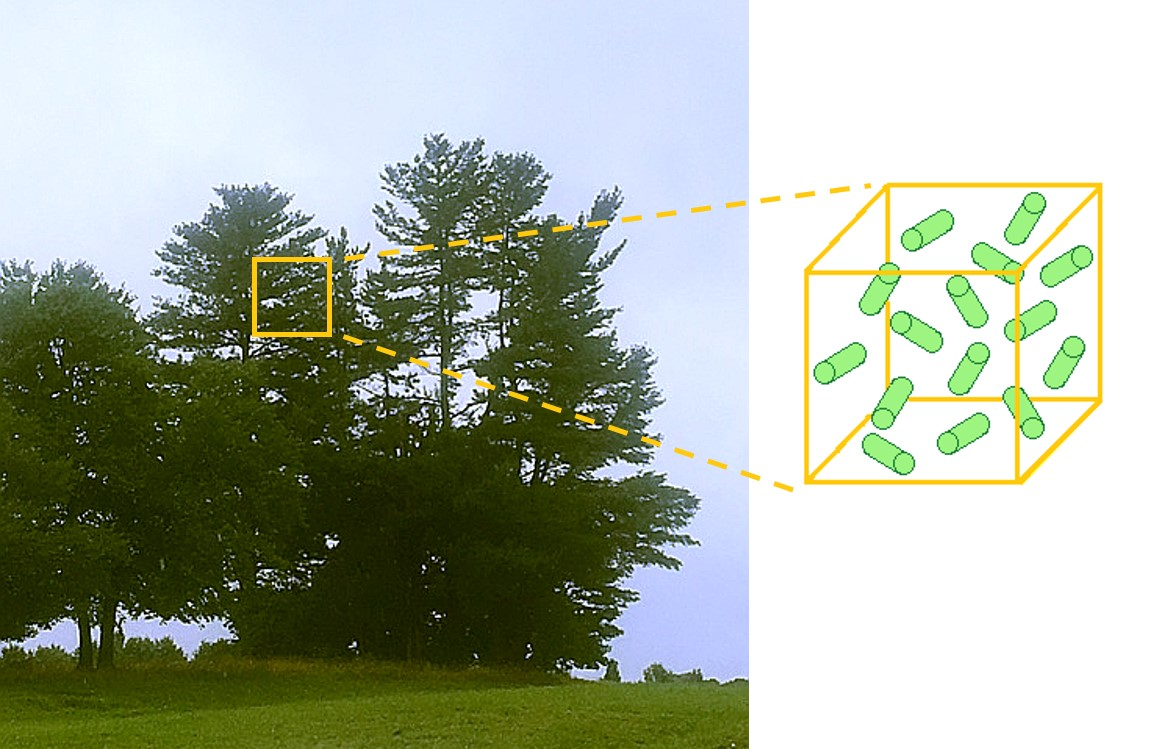
\includegraphics[width=1.0\linewidth]{Picture1.jpg}
	\caption{Vegetation translation to multi-component model}
	\label{fig:Canopymod}
\end{figure}

Equation~(\ref{eq:DragForce}) can be recast in an equivalent form that is more useful for describing vegetation drag~\cite{Mueller2014}:
\begin{equation}
\label{eq:DragForcea}
F  = \frac{\rho}{2} C_{\rm d} \, C_{\mathrm{s}} \, \beta \, \sigma \, U^2
\end{equation}
where $C_{\mathrm{s}}$ is a shape factor defined in this case as the average ratio of the projected area to surface area of the vegetative elements, $\beta$ is the ratio of the volume occupied by vegetation to the volume of the grid cell, $V$, and $\sigma$ is an average surface area to volume ratio of the vegetative elements. Some of the terms are difficult to measure, such as the shape factor and surface to volume ratio, but collectively these terms may be combined to form a parameter that resembles an absorption coefficient:
\begin{equation}
\label{eq:Kappa}
\kappa = C_{\mathrm{s}} \, \beta \, \sigma
\end{equation}
$\kappa$ can be determined by measuring the projected area of light passing a distance $L$ through the vegetation. The relative area of light, or ``free-area coefficient'', is defined by the relation:
\begin{equation}\label{eq:WhiteFraction}
W = {\rm e}^{-\kappa L}
\end{equation}
In the experiments, the cross-section of a small wind tunnel is filled with various amounts and types of vegetation to determine the drag coefficient for the following simplified model:
\begin{equation}\label{eq:Pressure}
F \equiv \frac{\Delta P}{L}  = \frac{\rho}{2} \, C_{\rm d} \, \kappa \, U^2
\end{equation}
\pagebreak


\section{Description of Experiments}
\label{sec:Experiments}


\subsection{Sample Preparation}
\label{ssec:SamplePrep}

The vegetation chosen for this work was a Bakers Blue Spruce ({\em Picea pungens `Bakeri'}), an Evergreen Distylium (Distylium `PIIDIST-I'), a Gold Rider Leyland Cypress ({\em Cupressocyparis leylandii `Gold Rider'}), a Kimberly Queen Fern ({\em Nephrolepis obliterata `Kimberly Queen'}), a Blue Shag Eastern White Pine ({\em Pinus strobus `Blue Shag'}), and a Robin Red Holly ({\em Ilex opaca}). Each sample was chosen based on its local availability. Leaf shapes were varied, including needle, elliptic, scale, and ovate.

The plant samples were cut into 0.5~\si{m} by 0.5~\si{m} by 0.5~\si{m} cubes using a guiding frame (Fig.~\ref{fig:Sampleprep}). The samples completely filled the cross section of the wind tunnel forcing the flow to move through the vegetation as opposed to around it. To easily distinguish the front, back, left, and right side of the cube-shaped vegetation, each side was designated Position A, B, C, or D (Fig.~\ref{fig:Vegpos}). After its initial cut, image analysis, wind tunnel measurements, and water displacement testing were conducted in subsequent order. In some cases, samples were pruned and tested again. In the case of the Bakers Blue Spruce, Gold Rider Leyland Cypress, and Robin Red Holly, four prunings were made with the final one being the removal of all leaves.

\begin{figure} [!]
	\centering 	
	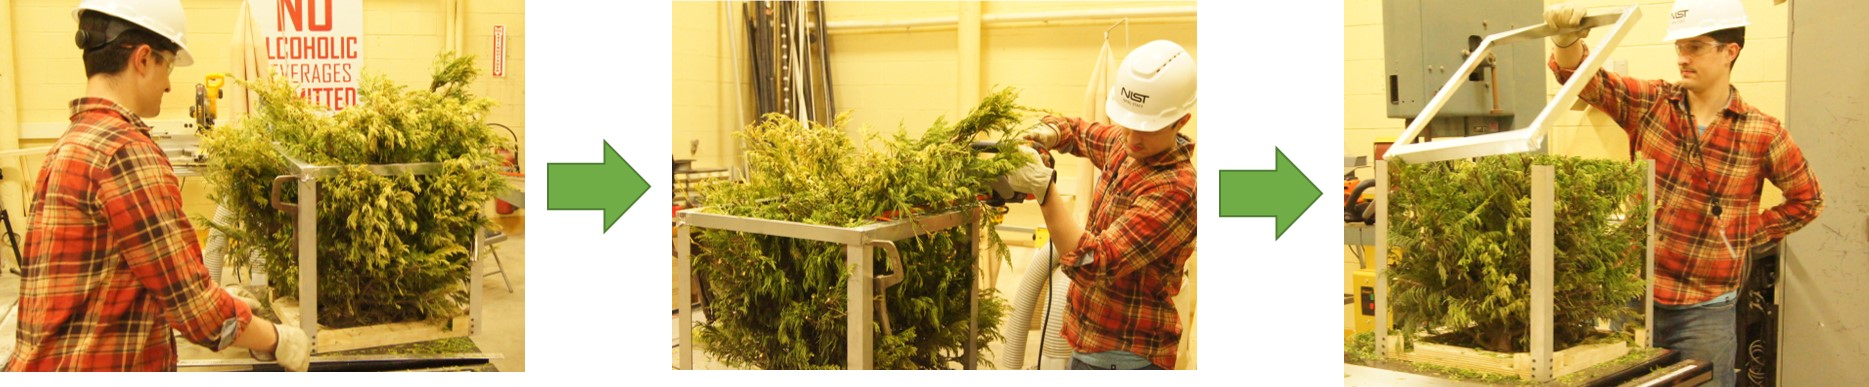
\includegraphics[height=8.in,keepaspectratio]{Picture2.jpg}
	\caption{Cutting procedure of vegetation samples}
	\label{fig:Sampleprep}
\end{figure}
\begin{figure} [!]
	\centering 	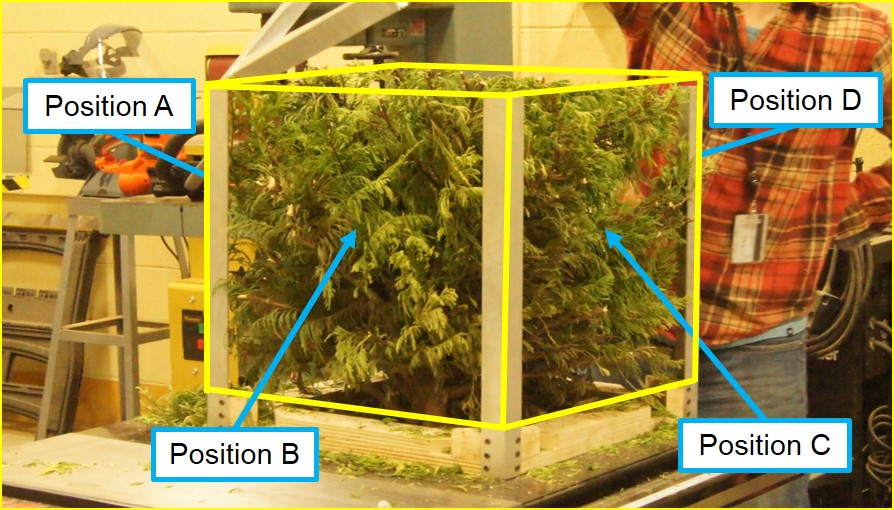
\includegraphics[width=1.0\linewidth]{Picture3.jpg}
	\caption{Prepared vegetation sample's designated orientation}
	\label{fig:Vegpos}
\end{figure}

\subsection{Determining the Free-Area Coefficient via Photography}
\label{ssec:Free-Area Coef. Photo}

The free-area coefficient was determined by placing each vegetation sample on a table located between a large white backdrop and a 0.5~m by 0.5~m cardboard frame, the same dimensions as the tunnel cross section (Fig.~\ref{fig:ImgAnaly}). For each sample cut and position, the projected area was photographed. All images were captured using a Nikon D5600 camera placed on a tripod located approximately 3.6~\si{m} away from the sample. The white backdrop was illuminated using a collection of incandescent and LED lights.

\begin{figure} [!h]
	\centering 	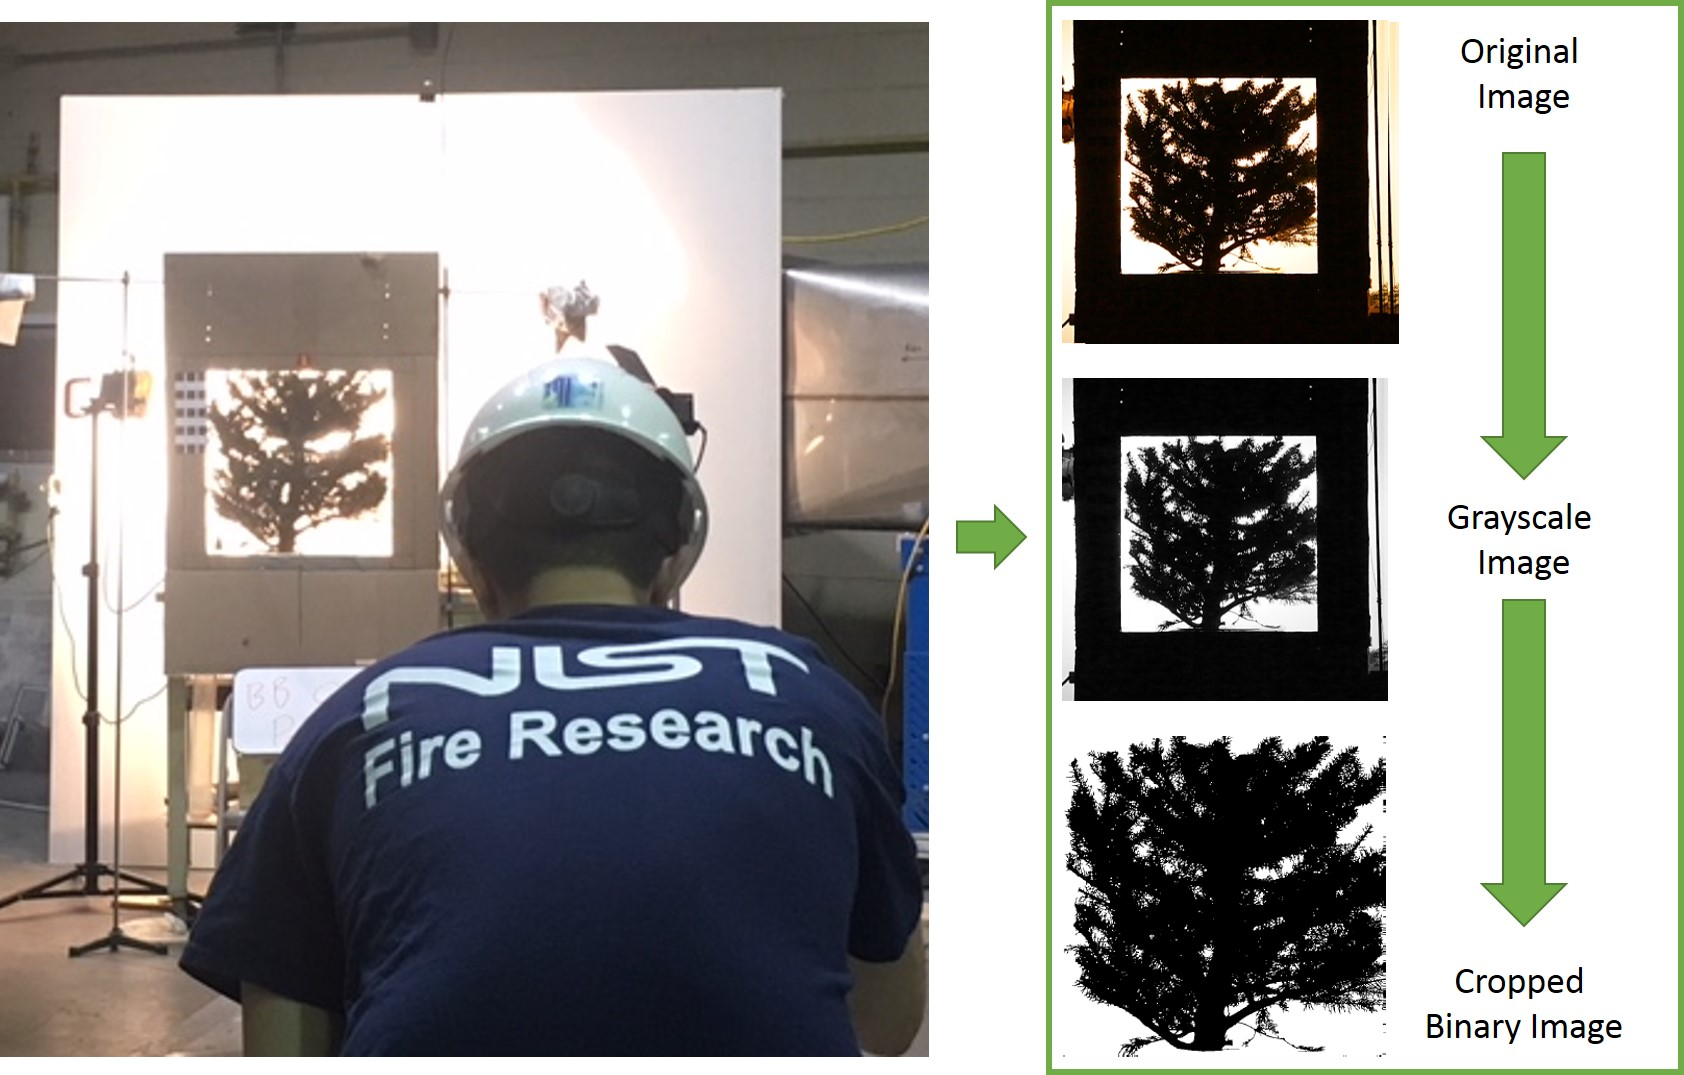
\includegraphics[width=1.0\linewidth]{Picture5.jpg}
	\caption[Setup for photographing vegetation samples]{Setup for photographing vegetation samples (left) and the post-processing procedure for analyzing images (right)}
	\label{fig:ImgAnaly}
\end{figure}

The images were processed using MATLAB's Image Processing Toolbox. Imported colored images were first converted into a grey scale and then a binary (black and white) image using a pre-set threshold level. The binary images were then cropped within the cardboard frame to eliminate non-vegetative substances and to evaluate the projected image of the vegetation exclusively. Once the projected image was obtained, a pixel count was conducted to determine the free-area coefficient of the vegetation, $W$. Once obtained, the free-area coefficient was used to calculate the absorption coefficient, $\kappa$, from Eq.~\ref{eq:WhiteFraction}.

A Type B, or epistemic, uncertainty of the free-area fraction and absorption coefficients was established using the same photography method and is described in further detail in Appendix~\ref{ssec:FAACUncertainty}.

\subsection{Description of the Wind Tunnel}
\label{ssec:headingscap}

Pressure loss measurements were obtained in a wind tunnel test section with a cross-sectional area of 0.5~\si{m} by 0.5~\si{m} and a length of 2~\si{m}. An image and schematic diagram of the wind tunnel setup is shown in Fig.~\ref{fig:WindtunnelPic}. The volume flow through the tunnel was measured upstream of the vegetation using a Rosemont~485 Annubar. The pressure drop across the vegetation was measured using an MKS Baratron Type 220D pressure transducer with a range of 0 to 133~Pa (1~torr). The air flow was provided by a 0.91~m axial fan controlled by a variable frequency drive and monitored using the Annubar. Air density was calculated from the tunnel's internal temperature measured with a Type-K thermocouple. Each sample configuration was subjected to nine different fan speeds ranging from 0 to 88~\% of the full-scale fan speed. The fan speed was not run at full scale due to the risk of exceeding the pressure transducer's pressure limitations. Data was sampled at 90~\si{Hz} for a 30~\si{s} period while maintaining a constant fan speed.

\begin{figure} [!]
	\centering 	
    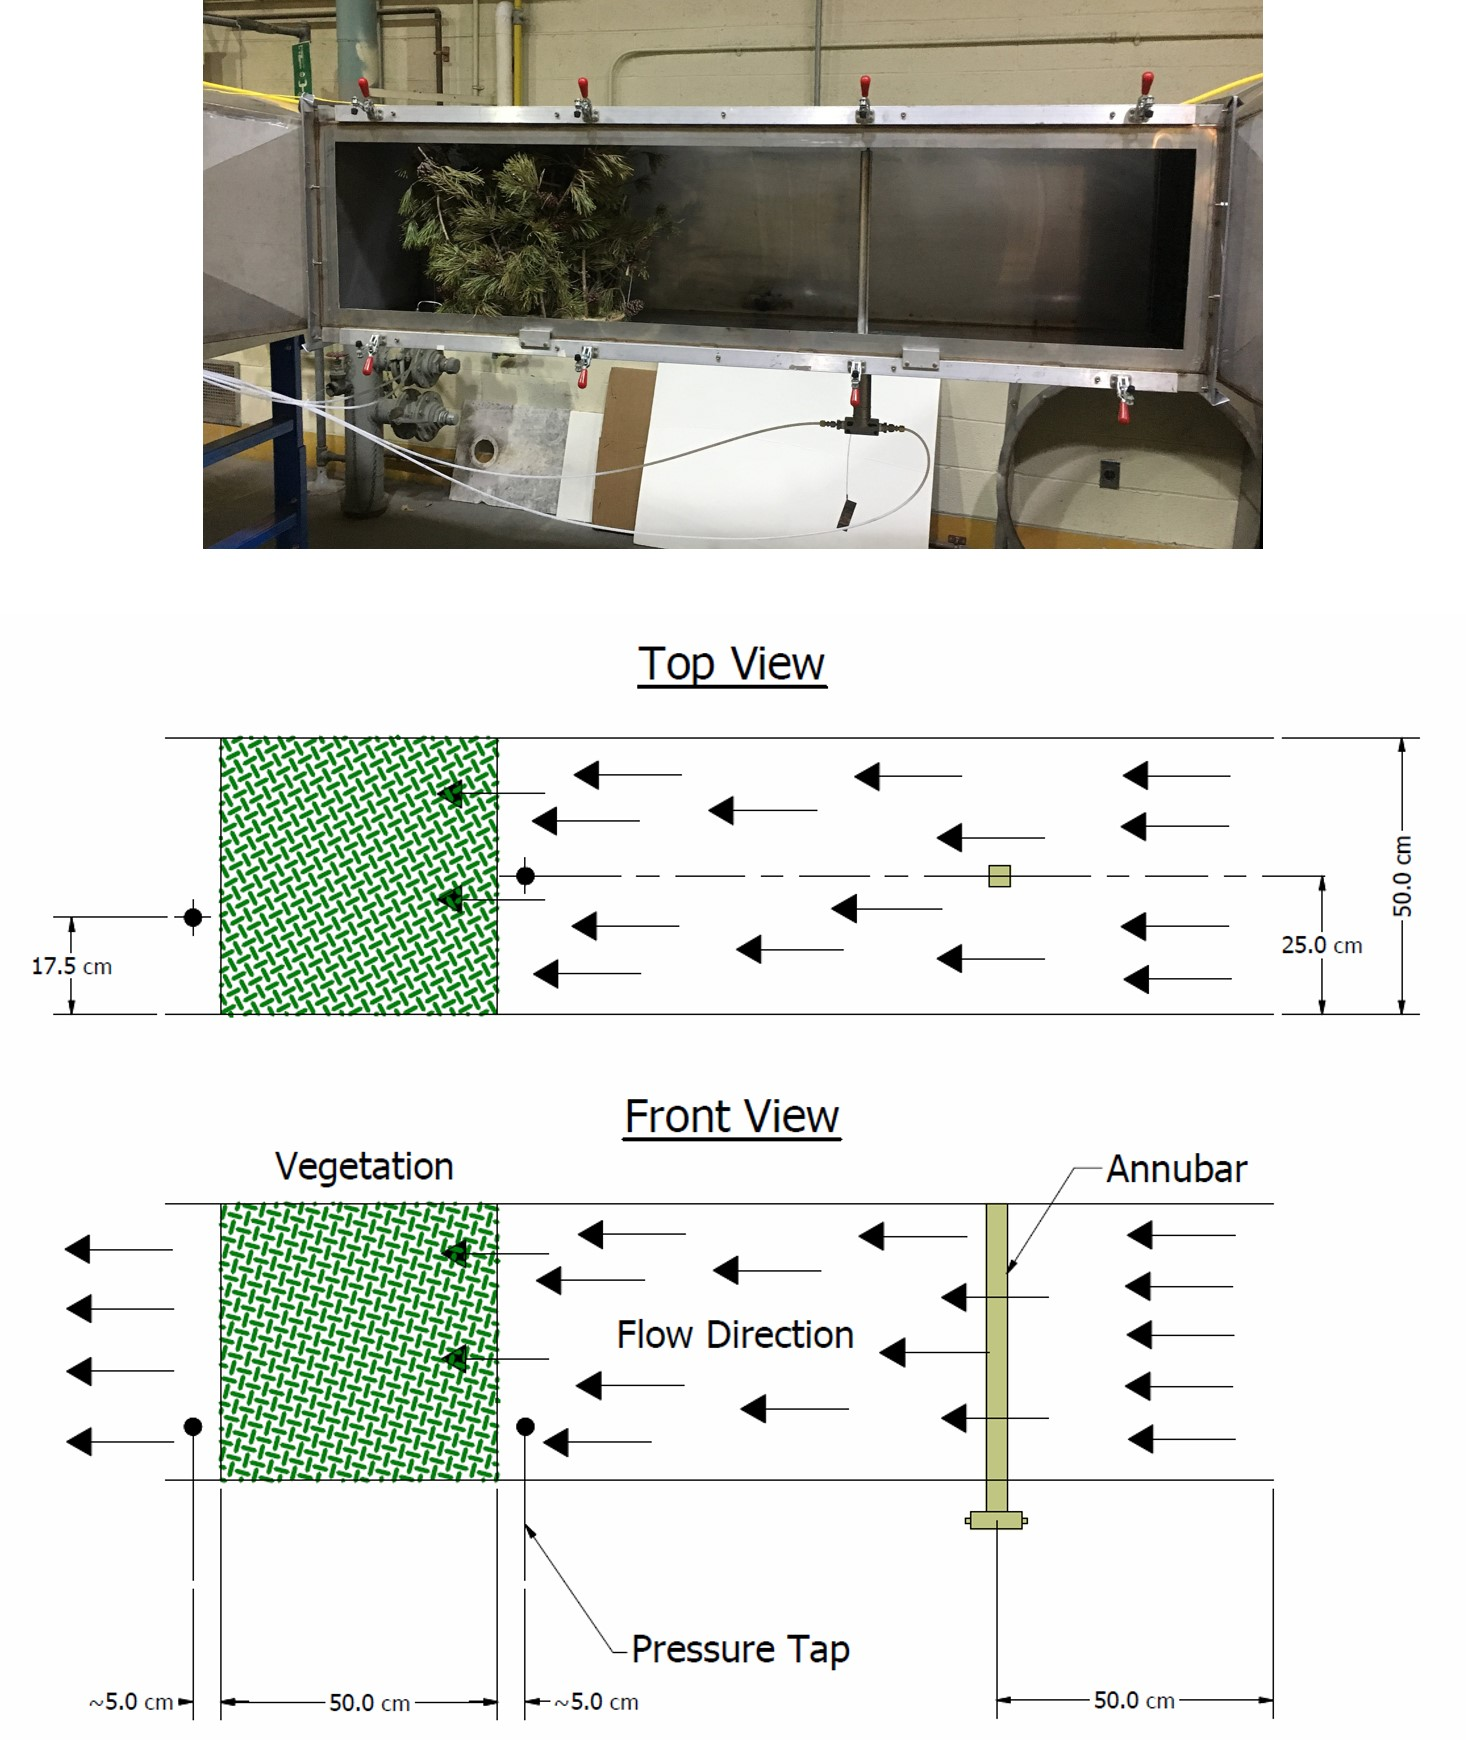
\includegraphics[width=\textwidth,keepaspectratio]{Picture6a.jpg}
	\caption[Wind tunnel experimental setup]{Wind tunnel experimental setup with top and front schematic drawings }
	\label{fig:WindtunnelPic}
\end{figure}

%\begin{figure} [!]
%	\centering 	
%    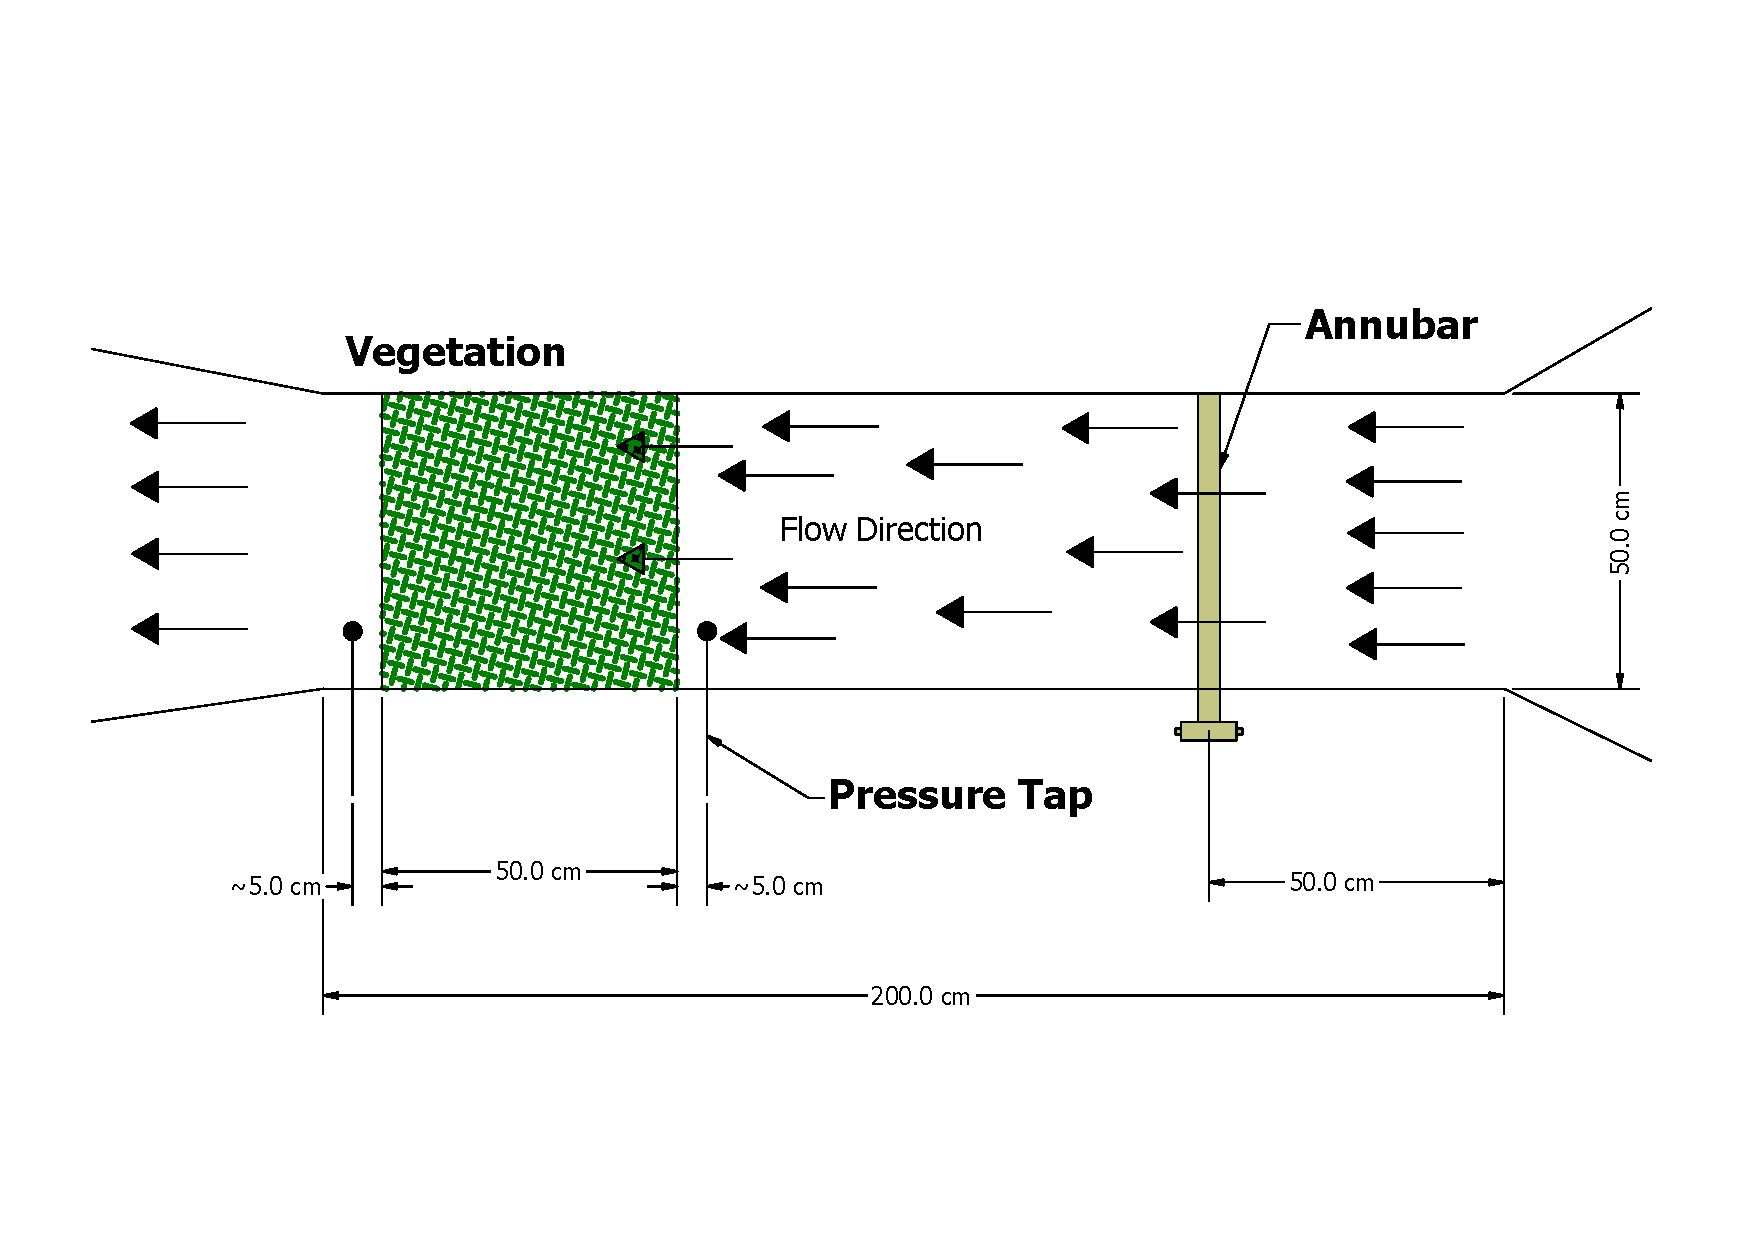
\includegraphics[width=\textwidth,keepaspectratio]{Drawing1.pdf}
%	\caption{Schematic diagram of the wind-tunnel experimental setup}
%	\label{fig:WindtunnelSch}
%\end{figure}

Once a set of measurements were taken at all fan speeds, the wind tunnel was shut off for approximately 5~\si{min}, and then the measurements were repeated. All measurements were repeated three times for each vegetation configuration. The variance homogeneity of the replicate measurements was tested using Hartley's F\textsubscript{max} test. If it was found that the data sets were homogenous, then the measurements were averaged.

An uncertainty analysis was conducted for the pressure and air density measurements and the subsequently determined velocities and drag coefficients.The characterization of the uncertainty for each parameter is provided in Appendix~\ref{sec:Uncertainty}.

\subsection{Determining the Volume of Vegetation via Water Displacement}
\label{ssec:waterdisp}

The volume of the vegetation was measured after a sample cut. The extracted vegetation was separated into branches and leaves and put into cloth mesh bags of known mass and volume, weighed\footnote{The mass was measured to estimate the water absorbed by the sample. The volume of water absorbed was subtracted from the volume of vegetation measured from the beaker.}, and submerged in a bucket. The displaced water flowed through a spout and into a beaker (Fig.~\ref{fig:wdt}). The measurement was repeated three times for each sample. The solid fraction, $\beta$, was calculated by dividing the average sample volume by the volume it occupied (0.5~\si{m} $\times$ 0.5~\si{m} $\times$ 0.5~\si{m} = 0.125~\si{m^{3}}). A combined Type A, or aleatoric, and Type B uncertainty was established for solid fraction parameter and is described in Appendix~\ref{sec:Uncertainty}.

\begin{figure} [!]
	\centering 	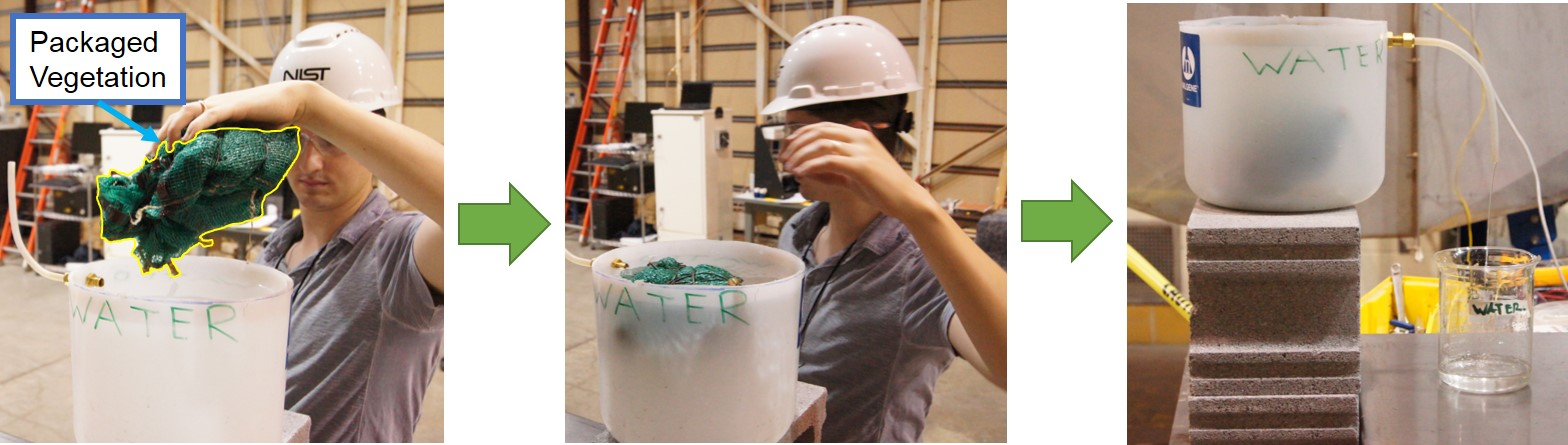
\includegraphics[height=0.95\textheight,keepaspectratio]{Picture7.jpg}
	\caption{Procedure of the water displacement test}
	\label{fig:wdt}
\end{figure}

\pagebreak



\section{Results}
\label{sec:results}

The key results of this work are the relationship between the absorption coefficient and solid fraction and more importantly the drag coefficient derived from the measurements made in the Image Analysis and Wind Tunnel Experiments.

\subsection{Relationship between the absorption coefficient $\kappa$ and solid fraction $\beta$ }

Figure~\ref{fig:betavkappa} presents the relationship between the absorption coefficient and solid fraction of all sample configurations. The symbols indicate the measured values while the dotted lines represent a linear regression fit. Each line represents a particular type of vegetation that has been pruned, reducing both its volume fraction its projected free-area coefficient, $W$, and corresponding the absorption coefficient, $\kappa$. There ought to be a linear relationship between $\kappa$ and $\beta$ if the shape factor, $C_{\rm s}$, and surface to volume ratio, $\sigma$ are constant, as shown in (Eq.~\ref{eq:Kappa}). However, this is not the case when the vegetative components are not uniform in size. Take, for example, the Robin Red Holly data shown in Fig.~\ref{fig:betavkappa}. As the solid fraction decreases, the absorption coefficient should approach zero, as demonstrated by most samples. As the leaves of the Robin Red Holly were pruned, its absorption coefficient, $\kappa$, decreased significantly even though its volume fraction did not, owing to the fact the ratio of branch to leaf volume of the Robin Red Holly is substantially higher than the other plant species, as shown in Table~\ref{tab:RatioTable},  As a result, the free-surface area, $W$, decreases from the removal of leaves, thus reducing the absorption coefficient, while still maintaining a relatively consistent solid fraction due to the significant volume contribution of the branches.

\begin{figure}[!]
	\centering 	
    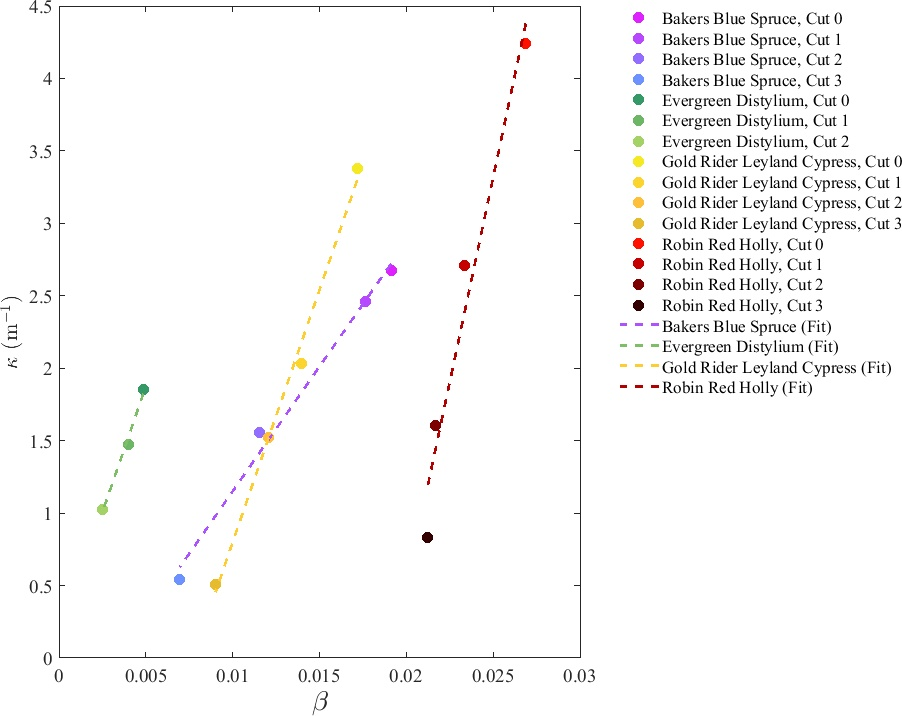
\includegraphics[width=1\linewidth]{Picture12.jpg}
	\caption[Comparison of absorption coefficient, $\kappa$, and solid fraction, $\beta$]{Calculated absorption coefficients ($\kappa$) of vegetation sample configuration plotted against their corresponding solid fractions ($\beta$)}
	\label{fig:betavkappa}
\end{figure}



\begin{table}[!]
\caption[Branch and leaf volume ratio of vegetation samples]{Branch and leaf volume ratio of vegetation samples with mulitple cut iterations}
\label{tab:RatioTable}
\centering
	
	\begin{tabular}{cccccc}	
			\hline
\rule{0pt}{14pt}\textbf{Sample}	&\textbf{Cut}	& ${\textfrac{Branch Volume}{Leaf Volume}}$ 	&\textbf{Sample}			&	\textbf{Cut}	& $\textfrac{Branch Volume}{Leaf Volume}$	\\
\hline
\\[0.01cm]
Bakers Blue Spruce			&	0		&        1.1							&Gold Rider Leyland Cypress	&	0		&	1.5						\\
					&	1		& 	1.3							&					&	1		&	2.2						\\
					&	2		& 	1.5							&					&	2		&	3.0						\\
					&	3		&	N/A							&					&	3		&  	N/A 						\\
					&			&								&					&			&       							\\
Evergreen Distylium			&	0		&	1.0							&Robin Red Holly			&	0		&	11						\\
					&	1		&	1.4							&					&	1		&	16						\\
					&	2		&	3.3							&					&	2		&	47						\\
					&			&								&					&	3		&        N/A 						\\
\\[0.005cm]
\hline														

\end{tabular}
\end{table}

\pagebreak


\subsection{Vegetation Canopy Drag Coefficients}
\label{ssec:headingscap}

Figure~\ref{fig:DPvU(Overall)} displays the relationship between the freestream velocity and the pressure drop for each sample configuration. The results demonstrate the expected quadratic relationship. Replotting the data as shown in Fig.~\ref{fig:DPoveraf(Overall)} yields the drag coefficient for each sample configuration as determined by calculating the slope of each line of data points. No linear regression fitting was observed to have a coefficient of determination value less than 0.98, indicating a close representation of the fitted regression line to the measured data. A summary of all 68 calculated drag coefficients and their respective uncertainties are presented in Table \ref{tab:SumTable}.

\begin{sidewaysfigure} [!]
	\centering
	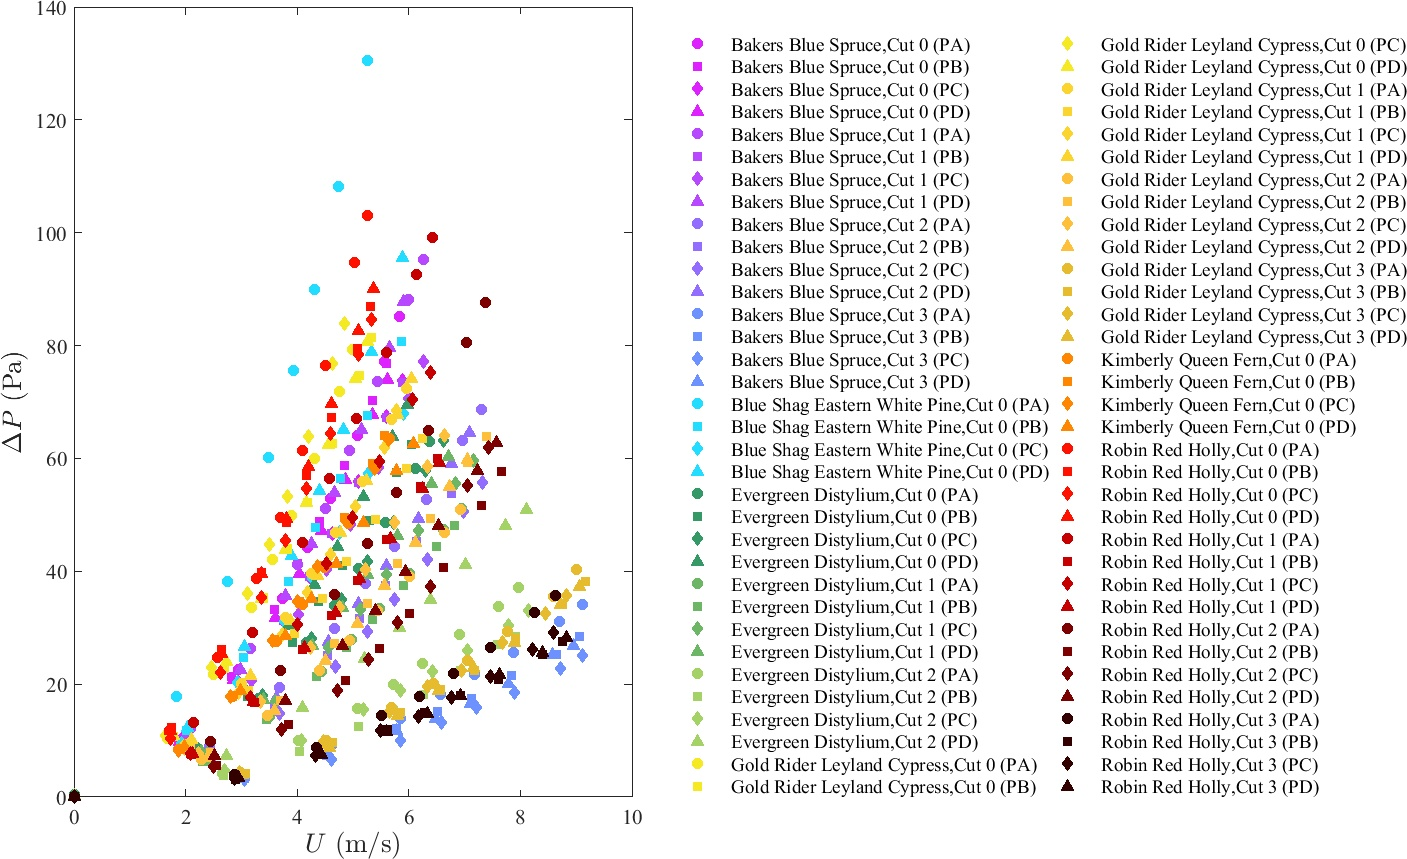
\includegraphics[width=\textwidth,keepaspectratio]{Picture8.jpg}
	\caption[Differential pressure measurements of vegetation samples]{Differential pressure measurements of vegetation samples subjected to a range of freestream velocities}
	\label{fig:DPvU(Overall)}
\end{sidewaysfigure}

\begin{sidewaysfigure}[!]
	\centering
	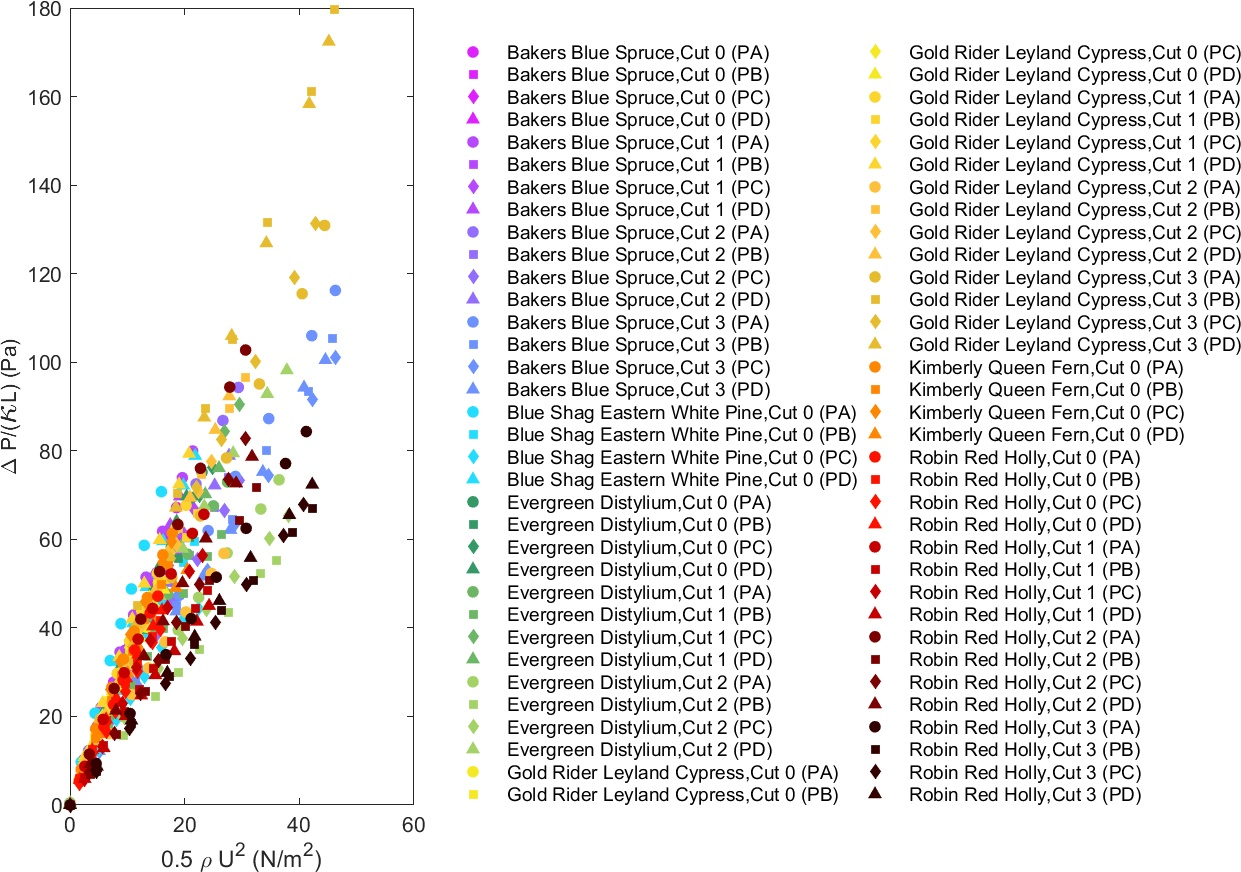
\includegraphics[width=\textwidth,keepaspectratio]{Picture9.jpg}
	\caption{Differential pressure measurements of vegetation samples over ($\kappa \, L$) vs. dynamic pressure}
	\label{fig:DPoveraf(Overall)}
\end{sidewaysfigure}

The distribution of all sample configurations' drag coefficient is shown in Fig.~\ref{fig:Histogram}. A Kolmogorov-Smirnov test (K-S test) was implemented to test the normality of the drag coefficient data. The K-S test determined that the drag coefficients of all sample configurations do not significantly vary from normality ($D(68)=\,0.09$)\footnote{The $D$ refers to the Kolmogorov-Smirnov test statistic, the 68 in brackets is the degrees of freedom (df), and the 0.09 is the actual K-S test statistic.}. The normal distribution of the data is further supported by the ``bell curve'' fitting displayed in  Fig.~\ref{fig:Histogram}. The average drag coefficient of all sample configurations was determined to be 2.8 with a standard deviation of 0.6.

\begin{figure}[!h]
	%\centering 	
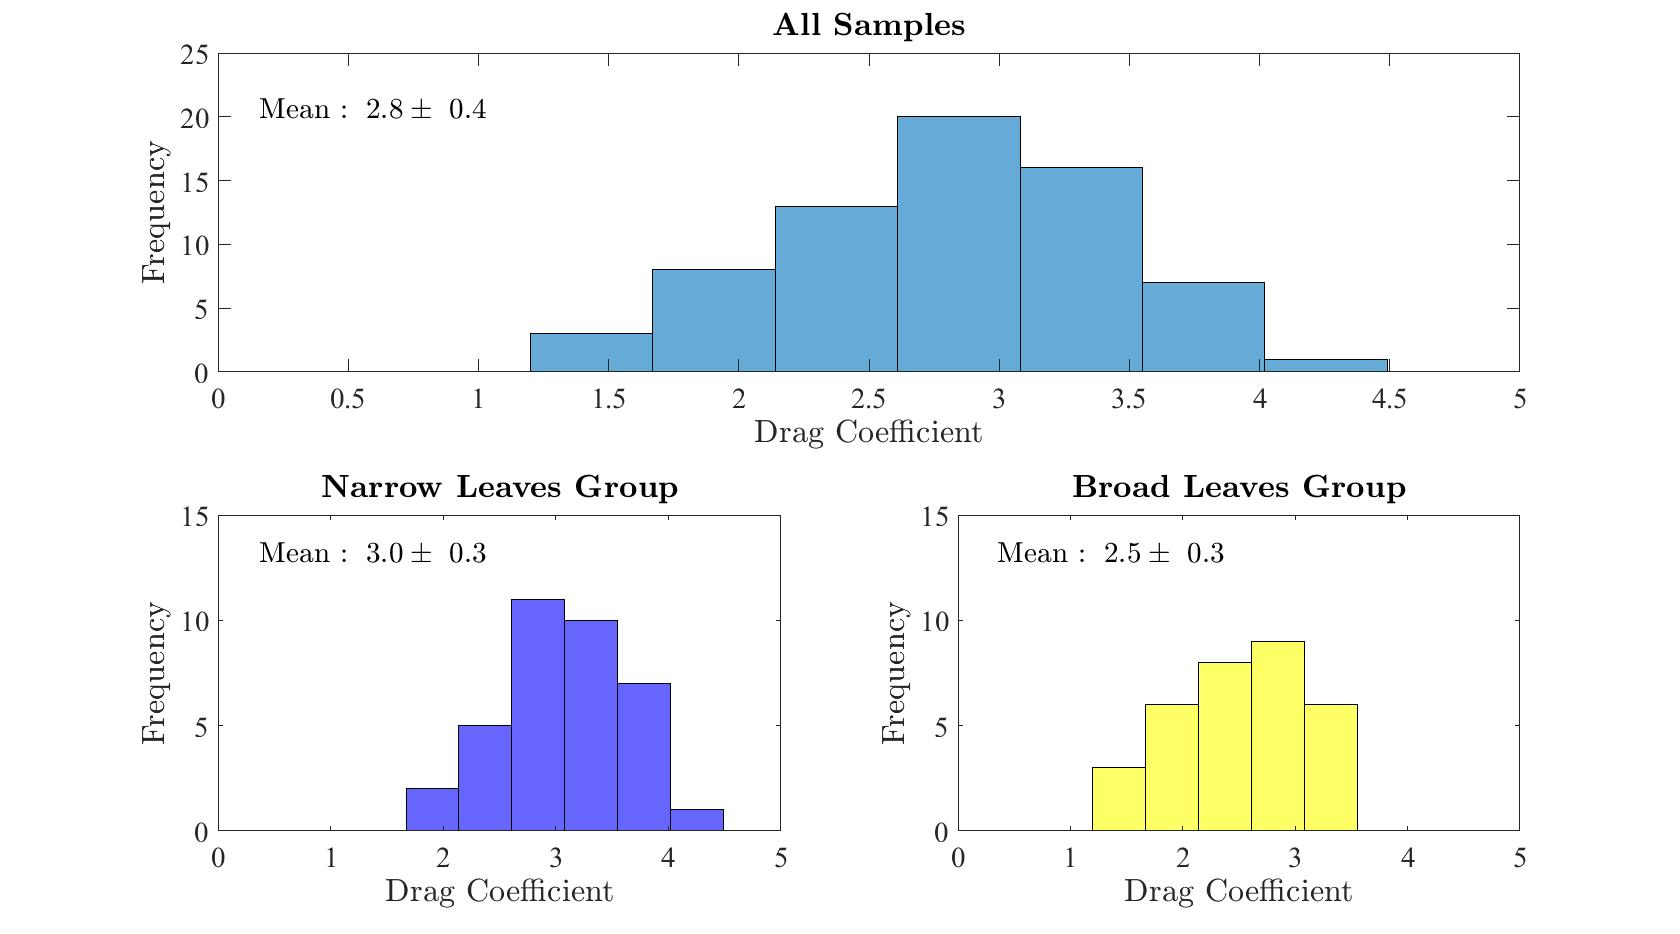
\includegraphics[width=\textwidth,keepaspectratio]{Picture11.jpg}
	\caption[Distribution of drag coefficients]{Distribution of vegetation samples drag coefficients with noted mean and standard deviation values}
	\label{fig:Histogram}
\end{figure}

\begin{table}
\caption{Drag Coefficient Summary of Vegetation Samples}
\label{tab:SumTable}
\centering

	\footnotesize
	\begin{tabular}{cccccccccc}	
			\hline
\textbf{Sample}		&	\textbf{Cut}	&\textbf{Position}& $C_{\rm d}$ 	&\textbf{Uncertainty}	&\textbf{Sample}	&	\textbf{Cut}	&\textbf{Position}& 	\textbf{$C_{\rm d}$ }&\textbf{Uncertainty}\\
\hline
\\[0.05cm]
Blue Spruce				&	0	&	A	& 	3.6	&	0.4				& Cypress       		&	0	&	A	& 	3.0	&	0.4	\\
					&		&	B	& 	3.2	&	0.4				&				&		&	B	& 	3.3	&	0.4	\\
					&		&	C	& 	3.1	&	0.4				&				&		&	C	& 	3.4	&	0.5	\\
					&		&	D	& 	3.0	&	0.4				&				&		&	D	& 	3.0	&	0.4	\\
					&	1	&	A	& 	3.7	&	0.4				&				&	1	&	A	& 	3.3	&	0.4	\\
					&		&	B	& 	3.0	&	0.4				&				&		&	B	& 	2.9	&	0.3	\\
					&		&	C	& 	3.1	&	0.3				&				&		&	C	& 	3.3	&	0.4	\\
					&		&	D	& 	3.6	&	0.4				&				&		&	D	& 	3.8	&	0.4	\\
					&	2	&	A	& 	3.2	&	0.3				&				&	2	&	A	& 	2.1	&	0.2	\\
					&		&	B	& 	2.7	&	0.3				&				&		&	B	& 	3.2	&	0.3	\\
					&		&	C	& 	2.5	&	0.3				&				&		&	C	& 	3.1	&	0.3	\\
					&		&	D	& 	2.8	&	0.3				&				&		&	D	& 	3.3	&	0.3	\\
					&	3	&	A	& 	2.5	&	0.3				&				&	3	&	A	& 	2.9	&	0.4	\\
					&		&	B	& 	2.3	&	0.4				&				&		&	B	& 	3.8	&	0.5	\\
					&		&	C	& 	2.2	&	0.4				&				&		&	C	& 	3.0	&	0.4	\\
					&		&	D	& 	2.3	&	0.4				&				&		&	D	& 	3.8	&	0.5	\\
					&		&		& 		&					&				&		&		& 		&		\\
White Pine	       			 &	0	&	A	& 	4.0	&	0.6				& Fern	       		 &	0	&	A	& 	3.2	&	0.4	\\
					&		&	B	& 	2.5	&	0.3				&				&		&	B	& 	2.8	&	0.4	\\	
					&		&	C	& 	1.9	&	0.3				&				&		&	C	& 	3.0	&	0.4	\\
					&		&	D	& 	3.4	&	0.4				&				&		&	D	& 	2.4	&	0.3	\\
					&		&		& 		&					&				&		&		& 		&		\\
Distylium				&	0	&	A	& 	3.2	&	0.3				&Red Holly			&	0	&	A	& 	3.1	&	0.4	\\
					&		&	B	& 	2.9	&	0.3				&				&		&	B	& 	2.6	&	0.3	\\
					&		&	C	& 	3.1	&	0.3				&				&		&	C	& 	2.5	&	0.3	\\
					&		&	D	& 	3.4	&	0.4				&				&		&	D	& 	2.7	&	0.3	\\
					&	1	&	A	& 	2.7	&	0.3				&				&	1	&	A	& 	2.8	&	0.2	\\
					&		&	B	& 	2.3	&	0.3				&				&		&	B	& 	2.0	&	0.2	\\
					&		&	C	& 	3.1	&	0.3				&				&		&	C	& 	2.5	&	0.2	\\
					&		&	D	& 	2.9	&	0.3				&				&		&	D	& 	1.8	&	0.2	\\
					&	2	&	A	& 	2.0	&	0.3				&				&	2	&	A	& 	3.4	&	0.2	\\
					&		&	B	& 	1.5	&	0.2				&				&		&	B	& 	2.2	&	0.2	\\
					&		&	C	& 	1.7	&	0.2				&				&		&	C	& 	2.7	&	0.2	\\
					&		&	D	& 	2.6	&	0.3				&				&		&	D	& 	2.5	&	0.2	\\
					&		&		& 		&					&				&	3	&	A	& 	2.1	&	0.2	\\
					&		&		& 		&					&				&		&	B	& 	1.6	&	0.2	\\
					&		&		& 		&					&				&		&	C	& 	1.6	&	0.2	\\
					&		&		& 		&					&				&		&	D	& 	1.7	&	0.2	\\
\\[0.05cm]
\hline														

\end{tabular}
\end{table}

To determine if the average drag coefficient depends on the type of vegetation a one-way analysis of variance (ANOVA) was implemented on the drag coefficients of the different vegetation samples. The analysis yielded a significant variation among the species ($F(5,62)=4.88$, $p=7.97 \times 10^{-4}$)\footnote{The $F$ refers to the statistic obtained from the F-test conducted in the ANOVA, the 5 and 62 in brackets represent the degrees of freedom, and the 4.88 is the actual F statistic derived from the ANOVA. The $p$ refers to the significance level determined from the F statistic and the $7.97 \times 10^{-4}$ is the actual p-value which was determined to be less than the chosen confidence level of 0.05, indicating a significant difference between the mean drag coefficients of the samples.} . A Tukey test was subsequently applied to if the species-specific average drag coefficients were significantly different from each other. The results showed one significant difference between the species' average drag coefficients: the Robin Red Holly and Gold-Rider Leyland Cypress. Despite this statistically significant difference, the average drag coefficients of the Robin Red Holly and Gold-Rider Leyland Cypress are both within one standard deviation away from the overall average drag coefficient, as demonstrated in Fig.~\ref{fig:Histogram},  and therefore is not large enough to have a practical implication. It can then be concluded that the variance of drag coefficients determined for each species is non-significant, meaning the overall average drag coefficient presented in Fig.~\ref{fig:Histogram} could be applied as a consistent drag coefficient for vegetation canopies in CFD models.

\section{Comparison Between Vegetation Data and Tube Bank Models}
\label{sec:comp}

In comparison to previous work~\cite{Cao2012,Jalonen2014,Mayhead1973,Gillies2002,Ishikawa2006}, the magnitude of the measured drag coefficients in this study is relatively large. As discussed in Section~\ref{sec:intro}, most previous studies have measured the wind resistance of a single plant or tree within a larger wind tunnel while this work considered a relatively homogenous distribution of vegetation within a tunnel. The interpretation of ``freestream'' velocity, shape factor, cross-sectional area, and so on, are often different in these studies, making it difficult to compare drag coefficients from one study to another. Within the field, there is no single definition of drag coefficient in regard to vegetation.

As a way to verify the accuracy of our wind tunnel measurements and the validity of our drag coefficient derivation, we considered a bank of regularly-spaced, staggered, vertical cylinders within our wind tunnel, using both actual steel rods and empirical results from Idelchick~\cite{Idelchick1994}. For each of the measured vegetation samples, a comparable configuration of vertical tubes was derived such that the volume fraction, $\beta$, absorption coefficient, $\kappa$, and characteristic diameter, $D$, match as closely as possible (see Table~\ref{tab:tube_parameters}). The characteristic diameter was calculated from Eq.~\ref{eq:Kappa} using the measured $\beta$ and $\kappa$ values and assuming a cylindrical shape factor ($C_{\mathrm{s}} = 1/\pi$). The expected pressure drop through the tube bank was either measured directly in the wind tunnel or taken from Idelchick (Eq.~\ref{eq:IdelchickTB}), and the corresponding drag coefficient was determined from Eq.~\ref{eq:Pressure}.
\begin{equation}
\label{eq:IdelchickTB}
\Delta P = \frac{\rho}{2}\,\frac{A\, \mathrm{Re}^{-0.25}}{W^{2}}\, U^2
\end{equation}
In Eq.~\ref{eq:IdelchickTB}, $A$ is defined as a geometric parameter determined from the tube bank configuration and Re is the Reynolds number which must be greater than 3000 for the empirical model to apply.

\begin{table}[!]
    \centering
    \caption{Parameters used in comparing vegetation with a comparable tube bank configuration}
    \label{tab:tube_parameters}
    \begin{tabular}{|c|c|c|c|c|c|c|c|c|}
    \hline
                                 & \multicolumn{2}{|c|}{$\beta$ (\%)} & \multicolumn{2}{|c|}{$\kappa$ (m$^{-1}$)} & \multicolumn{2}{|c|}{$D$ (mm)} &                             &                                  \\ \cline{2-7}
    \raisebox{1.5ex}[0pt]{Pos.}  & Veg.             & Tubes      & Veg.                 & Tubes              & Veg.              & Tubes      & \raisebox{1.5ex}[0pt]{Rows} & \raisebox{1.5ex}[0pt]{Tubes/Row} \\ \hline \hline
    \multicolumn{9}{|c|}{Gold Rider Leyland Cypress, Cut 2}                                                                                                                                                    \\ \hline
    A                            & 1.2            & 1.1      & 1.8                  & 1.7                & 8.5               & 9.5        & 4                           & 5                                \\ \hline
    B                            & 1.2            &1.2      & 1.3                  & 1.3                & 11.6              & 12.6       & 4                           & 3                                \\ \hline
    C                            & 1.2            & 1.3      & 1.7                  & 1.8                & 9.3               & 10.1       & 5                           & 4                                \\ \hline
    D                            & 1.2           & 1.2      & 1.3                  & 1.3                & 11.9              & 13.8       & 2                           & 5                                \\ \hline
        \multicolumn{9}{|c|}{Bakers Blue Spruce, Cut 2}                                                                                                                                                    \\ \hline
    A                            &1.2           & 1.1      & 1.5                  & 1.4                & 10.1              & 10.8       & 5                           & 3                                \\ \hline
    B                            & 1.2          & 1.1      & 1.6                  & 1.5                & 9.2               & 9.8        & 6                           & 3                                \\ \hline
    C                            & 1.2            & 1.1     & 1.5                  & 1.5                & 9.7               & 10.6       & 4                           & 4                                \\ \hline
    D                            & 1.2            & 1.2      & 1.6                  & 1.7                & 9.0               & 9.7        & 5                           & 4                                \\ \hline
    \end{tabular}
\end{table}

\begin{figure}[!]
	\centering 	
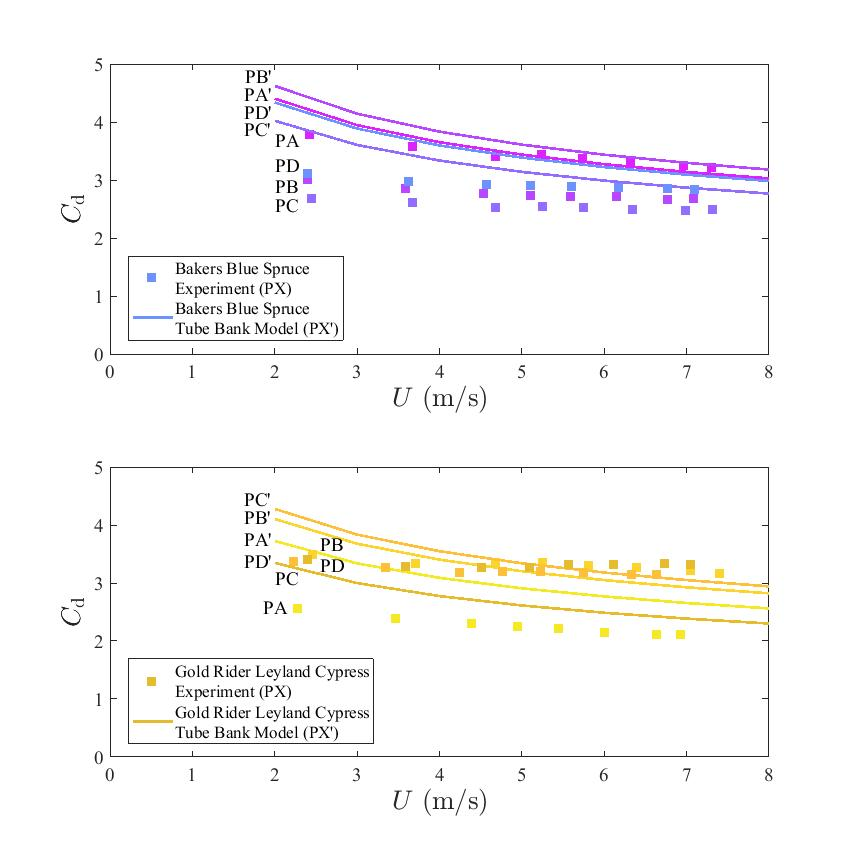
\includegraphics[width=1\linewidth]{Picture13.jpg}
	\caption[Drag Coefficient comparison between vegetation samples and tube bank configurations]{Drag Coefficient comparison between vegetation sample configurations (Bakers Blue Spruce, Cut 2 and Gold Rider Leyland Cypress, Cut 2) and thier corresponding tube bank configuration with respect to velocity}
	\label{fig:TBGR}
\end{figure}

Figure~\ref{fig:TBGR} compares the drag coefficients from the Gold Rider Leyland Cypress and Bakers Blue Spruce with their tube bank equivalents. While the match is not expected to be perfect given the difference in skin fraction, shape, and so on, the drag coefficients of each configuration is comparable.
\pagebreak

\section{Conclusion}

This report documents a series of experiments implemented to determine the absorption coefficient, pressure loss, and the solid fraction of different types of vegetation sample configurations. The primary objective of this work was to calculate the drag coefficients of ``bulk'' vegetation that can be incorporated into CFD models. In addition to establishing drag coefficients of ``bulk''  vegetation, notable findings regarding vegetation structure and similarities between drag coefficients of plant species were also discovered from this work. It cannot be concluded, however, that the findings from this work applies to all ``bulk'' vegetation, but exclusively to the samples studied in these experiments.

\begin{enumerate}
  \item The calculated absorption coefficient for each sample demonstrated a strong relationship with its corresponding solid fraction.
  \item The overall average drag coefficient of the bulk vegetation was found to be 2.8 with a standard deviation of 0.6. The differences between the average drag coefficients of different plant species were concluded to be non-significant suggesting that the overall average drag coefficient could be used as a constant value in CFD models of various plant types.
\end{enumerate}

\section*{Acknowledgments}

\noindent Matthew Bundy and Artur Chernovksy of the National Fire Research Laboratory assisted in conducting these experiments and in processing the data.   \\
%%%%%%%%%%%%%%%%%%%%%%%%%%%%%%%%%%%%%%%%%%%%%%%%%%%%%%%%%%%%%%%%%%%%
%   Acknowledgments not required
%%%%%%%%%%%%%%%%%%%%%%%%%%%%%%%%%%%%%%%%%%%%%%%%%%%%%%%%%%%%%%%%%%%%
\pagebreak
\section*{References}
\addcontentsline{toc}{section}{References}
\bibliographystyle{techpubs}
\bibliography{References}
\pagebreak

%%%%%%%%%%%%%%%%%%%%%%%%%%%%%%%%%%%%%%%%%%%%%%%%%%%%%%%%%%%%%%%%%%%%
%   Please use the techpubs BibTeX style when compiling bibliography, or follow the instructions on tinyurl.com/techpubsnist to format your .bib / .bbl file appropriately.
%%%%%%%%%%%%%%%%%%%%%%%%%%%%%%%%%%%%%%%%%%%%%%%%%%%%%%%%%%%%%%%%%%%%
%%%%%%%%%%%%%%%%%%%%%%%%%%%%%%%%%%%%%%%%%%%%%%%%%%%%%%%%%%%%%%%%%%%%
%   Authors who have supplemental materials should submit them when submitting their manuscripts for review. Supplemental materials may include computer code or data files associated with the paper. A brief description of the supplemental material must be included in the paper. A DOI will be assigned to the supplemental material and inserted into the paper by the Information Services Office.
%%%%%%%%%%%%%%%%%%%%%%%%%%%%%%%%%%%%%%%%%%%%%%%%%%%%%%%%%%%%%%%%%%%%

\appendix
\numberwithin{equation}{section}
\makeatletter
% "activate" the preparatory code, but for section-level headers only
\newcommand{\section@cntformat}{Appendix:\ }
\makeatother
\section{Uncertainty Analysis} \label{sec:Uncertainty}
\addcontentsline{toc}{section}{Appendix A: Uncertainty Analysis}

The drag coefficient was calculated using a combination of Eqs.~(\ref{eq:WhiteFraction}) and (\ref{eq:Pressure}):
\begin{equation}\label{eq:drag_coefficient}
  C_\mathrm{d} = \frac{-2 \, \Delta P}{\rho \, U^2 \, \ln \, W}
\end{equation}
where $\Delta P$ is the pressure drop across the vegetation sample, measured with a pressure transducer, $\rho$ is the air density, obtained via a temperature measurement and the ideal gas equation of state, $U$ is the average velocity of air through the wind tunnel, measured using an Annubar, and $W$ is the free area coefficient of the vegetation, measured using photography and image analysis. The uncertainty of the measured drag coefficient was estimated using the law of propagation of uncertainty:
\begin{equation}
\label{eq:DragUncertainty}
u_\mathrm{c} = \sqrt{{\left( \frac{\partial C_{\rm d}}{\partial \Delta P}\,u_{\scriptscriptstyle \Delta P} \right)}^2+{\left(\frac{\partial C_{\rm d}}{\partial \rho}\,u_{\scriptscriptstyle \rho}\right)}^2+{\left(\frac{\partial C_{\rm d}}{\partial U}\,u_{\scriptscriptstyle U}\right)}^2+{\left(\frac{\partial C_{\rm d}}{\partial W}\,u_{\scriptscriptstyle W}\right)}^2}
\end{equation}


\subsection{ Free-Area Coefficient }
\label{ssec:FAACUncertainty}

The uncertainty of the free-area coefficient was determined by measuring the projected areas of objects with known dimensions using the same photographic method described in Section~\ref{ssec:Free-Area Coef. Photo}. The standard deviation of the difference between the measured and true free-area coefficients was found to be $u_{\scriptscriptstyle W}=0.01$, which was treated as a Type B evaluation of standard uncertainty for all free-area coefficients of the vegetation samples.


\subsection{Pressure}
\label{ssec:PressUncertainty}

Two pressure transducers were used in this study. Transducer 1 measured the differential pressure across the vegetation while Transducer 2 measured the differential pressure across the Annubar. The Type A evaluation of standard uncertainty of the pressure difference, $\Delta P$, was taken as the standard deviation of the measurements made during a 30~s period, $s_{\scriptscriptstyle \Delta P}$. The Type B evaluation of standard uncertainty was determined from the calibration error sources of the pressure transducers and was found to be $u_{\rm \scriptscriptstyle cal}=1.4$~Pa and $u_{\rm \scriptscriptstyle cal}=1.5$~Pa for Transducers 1 and 2, respectively. The combined uncertainty was found via quadrature:
\begin{equation}
\label{eq:pressureuncertainty}
u_{\scriptscriptstyle \Delta P} = \sqrt{ u_{\rm \scriptscriptstyle cal}^2 + s_{\scriptscriptstyle \Delta P}^2}
\end{equation}


\subsection{Air Density}
\label{ssec:ADUncertainty}

The density of air was determined from the equation of state
\begin{equation}
   \rho = \frac{ 29 \, P }{8314 \, T}
\end{equation}
The combined standard uncertainty in the measured air temperature was XX~K. The combined standard uncertainty in the atmospheric pressure was XX~Pa. Therefore, the combined standard uncertainty in the air density was $u_{\scriptscriptstyle \rho}=YY$~kg/m$^3$.


\subsection{Velocity}
\label{ssec:VelUncertainty}

The average air velocity through the wind tunnel, $U$, was measured using an Annubar and calculated using the following formula:
\begin{equation}
\label{eq:Velocity}
U = K \, \sqrt{\frac{2 \, \Delta P}{\rho}}
\end{equation}
where $K$ is a flow coefficient and $\Delta P$ is the pressure difference measured by Transducer~2 discussed above. The standard uncertainty of the velocity was determined through the law of propagation of uncertainties:
\begin{equation}
\label{eq:Velocityuncertainty}
u_{\scriptscriptstyle U} = \sqrt{{\left( \frac{\partial U}{\partial \Delta P}\,u_{\scriptscriptstyle \Delta P} \right) }^2+{\left(\frac{\partial U}{\partial \rho}\,u_{\scriptscriptstyle \rho}\right)}^2}
\end{equation}


\subsection{Solid Fraction}\label{ssec:SFUncertainty}
The solid fraction of the vegetation, $\beta$, was determined using the water displacement testing described in Section~\ref{ssec:waterdisp}. The uncertainty of the solid fraction combined the Type A uncertainty of the repeated volume measurements and the Type B uncertainty in the resolution of the beaker used to measure the volume (5 ml) and Load Cell used to measure the mass (0.005 kg). The Type A uncertainty was calculated from the product of standard deviation of the repeated $\beta$ measurements and a coverage factor of 2, assuming a level of confidence of approximately 95~\%.

\begin{equation}
\label{eq:betauncertainty}
\mu_{\beta} = \sqrt{{(\mu_{B\,Res.})^2+(\mu_{L.C.,\,Res.})^2+(2\,S_{\beta})}^2}
\end{equation}


\end{document}
